\section{Внутренние форматы хранения данных}
\setcounter{figure}{0}

% The 3-Clause BSD License

В данной работе используется комбинация из различных структур данных, 
объединённых в единую систему.
Полная схема структур и их связей представленна на рис. \ref{overall_data_structure}

\begin{figure}[hpt!]
    \centering
    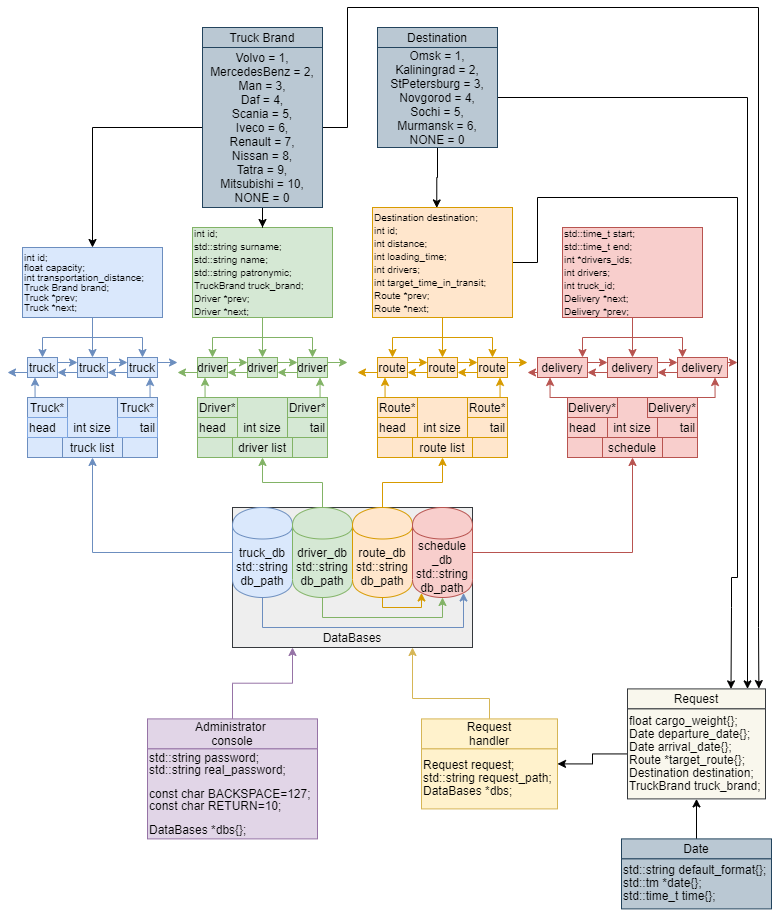
\includegraphics[width=1\linewidth]{photo/overall_data_structure}
    \caption{Обзорная диаграмма структур данных программы}
    \label{overall_data_structure}
\end{figure}

\newpage

\subsection{Структура данных двусвязный список}

В работе предпологается использование структуры данных "список".
Список --- структура данных, состоящая из элементов, 
содержащих помимо собственных данных ссылки на 
следующий и/или предыдущий элемент списка \cite{list_defenition}.

Для работы был вабран вариант с двунаправленым списком, 
где каждый узел имеет указатель на следующий и на предыдущий элементы.
Схема двунаправленного списка показана на рис. \ref{list_schema}.

\begin{figure}[hpt!]
    \centering
    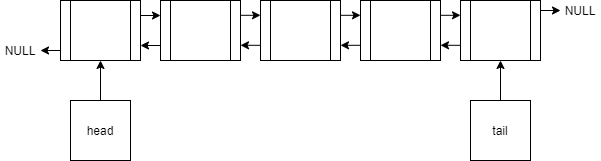
\includegraphics[width=1\linewidth]{photo/list_schema}
    \caption{Схема структуры данных двусвязный список}
    \label{list_schema}
\end{figure}

\subsection{TruckBrand}
\subsection{Destination}
\subsection{Truck}
\subsection{TruckList}
\subsection{TruckDataBase}
\subsection{Route}
\subsection{RouteList}
\subsection{RouteDataBase}
\subsection{Driver}
\subsection{DriverList}
\subsection{DriverDataBase}
\subsection{Delivery}
\subsection{Schedule}
\subsection{ScheduleDataBase}
\subsection{DataBases}
\subsection{AdministratorConsole}
\subsection{Date}
\subsection{Request}
\subsection{RequestHandler}
